\documentclass[conference]{IEEEtran}
\usepackage[T1]{fontenc}
\usepackage{times}
\usepackage{amsmath,amssymb,graphicx,booktabs}
\usepackage{multicol}
\usepackage[numbers,sort&compress]{natbib}
\usepackage[hidelinks]{hyperref}
\hypersetup{pdfauthor={},pdftitle={When Does Physical Diagnosis Compromise Robot Recovery?},pdfsubject={Anonymous manuscript}}
\newcommand{\K}{\mathcal K}
\newcommand{\A}{\mathcal A}
\newcommand{\B}{\mathcal B}
\newcommand{\E}{\mathbb E}
\newcommand{\ind}{\mathbb I}
\begin{document}
\title{When Does Physical Diagnosis Compromise Robot Recovery?}
\author{Author Names Omitted for Anonymous Review}
\maketitle
\begin{abstract}
A robot that probes a failed contact can learn how to recover while changing whether recovery remains possible. Does this effect matter beyond the time spent probing? We formulate recovery opportunity as the set of executable corrective policies that complete a task within a declared remaining budget. A matched physical probe--hold protocol measures loss of this set at a common deadline, distinguishes losing one correction from losing the entire repertoire, and evaluates the diagnostic information obtained. Recovery-aware diagnostic selection is a conventional contingent decision problem; we claim neither a new planning algorithm nor an advantage over a planner with the same objective. We specify a prospective contact-sensitive assembly study testing two materiality hypotheses: informative, constraint-compliant repertoire erasure in at least 10\% of eligible checkpoints, and at least five percentage points higher completion than constrained information-gain selection. A constructed equal-duration example establishes the logical distinction; existing cube executions establish only narrow source feasibility. Assembly source qualification and population validation remain outstanding. The proposed study can therefore distinguish physical loss, deadline dependence, catalogue dependence, and equivalence to existing task-aware decisions.
\end{abstract}

\section{Introduction}
A peg stops at the mouth of a fixture. An axial preload might reveal whether it is misaligned; a lateral dither might reveal a different contact response. Either interaction can also move the peg into a state from which the available correction no longer succeeds. Waiting consumes time too. To attribute a loss to diagnosis, one must compare these physical interactions with equal-duration holding, at the same remaining deadline and with the same corrective policies.

The question is: \emph{under which post-failure contact conditions does informative diagnosis remove recovery opportunities beyond elapsed time, and when does preserving those opportunities improve completion?} This is a question about a declared task, source distribution, controller catalogue, and budget. Remaining within an allowed state set does not establish that a task can still be completed. Conversely, failing one corrective policy does not establish that all recovery has become impossible.

\begin{figure}[t]
\centering
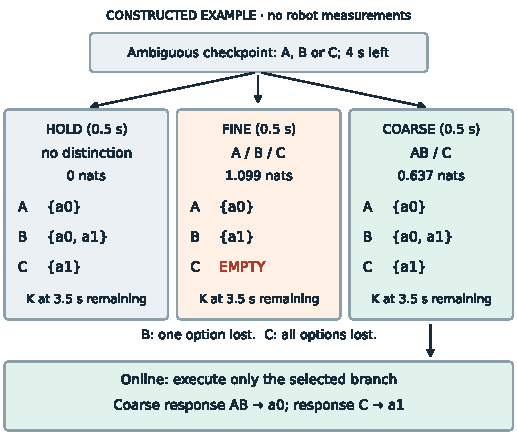
\includegraphics[width=\columnwidth]{figures/figure1.pdf}
\caption{Physical diagnosis changes uncertainty and future recovery options. The three equal-time branches and their option sets are \emph{constructed}, not measured robot outcomes. Fine diagnosis distinguishes all three worlds but erases the entire catalogue in C; in B it removes only one option. Coarse diagnosis preserves a response-dependent successful correction. Offline matched branches evaluate these contrasts; the online robot executes only its selected branch.}
\label{fig:thesis}
\end{figure}

Physical interaction as sensing is established \citep{bohg2017}. Active fault estimation can already combine information seeking with collision constraints \citep{ragan2024}; decision-aware tactile disambiguation can stop when hypotheses support a common grasp and can model contact disturbance \citep{wang2026}. Reversibility-aware control \citep{eysenbach2018,grinsztajn2021} and the distinction between identifiability and downstream terminal controllability \citep{kobayashi2026} also precede this work. Our proposed contribution is a \emph{time-controlled post-failure investigation} of recovery-option loss, coupled to decisions whose completion consequences can be measured against strong task-aware alternatives.

We formulate recovery opportunity as the set of executable corrective policies satisfying a task goal within a declared remaining budget. This supports a matched intervention protocol that separates diagnostic state changes from elapsed-time effects and distinguishes individual-option loss from entire-repertoire erasure. We use it to specify recoverability-aware diagnostic decisions and a controlled investigation of their completion, information, and effort tradeoffs in contact-sensitive manipulation. The resulting planner has an established belief-space formulation. A full-model planner optimizing the same objective should agree.

Two prospective hypotheses make the investigation falsifiable. \textbf{H1} predicts that a frozen information-seeking policy produces informative, constraint-compliant responses while erasing the declared repertoire relative to holding in at least 10\% of eligible checkpoints. \textbf{H2} predicts at least a five-percentage-point completion gain from accounting for post-probe opportunities, under the same model, sensors, actions, constraints, and time budget. These are proposed materiality margins, not observed effects. A finite example demonstrates possibility; the physical prevalence and policy benefit remain open.

\section{Recovery Opportunity and Diagnostic Decisions}
\subsection{A task-relative, time-relative set}
Let $s$ include physical state and relevant controller memory, $h$ be the legitimate observation history, and $\tau$ the remaining task time. Fix a finite catalogue $\A$ of executable feedback recovery policies. In a deterministic reference model, let $G(s,a,\tau)\in\{0,1\}$ indicate terminal task completion by policy $a$ within $\tau$. Define
\begin{equation}
\K_\tau(s)=\{a\in\A:G(s,a,\tau)=1\}.\label{eq:K}
\end{equation}
An empty set means failure of this catalogue within this budget, not impossibility for every controller. A policy may use permitted feedback during execution; its identifier denotes the entire frozen feedback policy rather than one open-loop command.

For nominal support $\B(h)$, an executable common choice requires
\begin{equation}
\operatorname{Common}_\tau(\B)=\bigcap_{s\in\B}\K_\tau(s)\ne\emptyset.\label{eq:common}
\end{equation}
Each state can have a nonempty set while this intersection is empty. This distinction motivates diagnosis: its response can determine which correction to execute. It also prevents an offline evaluator's knowledge of $s$ from becoming an online action oracle.

Physical constraints are separate. An admissible trajectory remains in a declared allowed set or satisfies specified sampled limits. It can nevertheless end with $\K_\tau(s)=\emptyset$. These limits are measured constraints, not a claim of general hardware safety. Recovery-policy path compliance is reported alongside terminal success; a successful but violating branch cannot establish compliant recovery.

\subsection{Diagnosis changes the state as well as the belief}
A probe $p$ consumes duration $d_p$, follows a trajectory $\xi_p(s)$, transitions to $T_p(s)$, and returns response $y=O_p(s,T_p(s),\xi_p(s))$. The state is augmented with any memory needed to make these mappings well defined. The updated support is
\begin{equation}
\B_{p,y}=\{T_p(s):s\in\B,\ O_p(s,T_p(s),\xi_p(s))=y\}.\label{eq:update}
\end{equation}
There is no reset between a probe and its recovery. The latter receives $\tau-d_p$, not a fresh task budget. In a stochastic model the joint kernel $P_p(ds',dy\mid s)$ replaces these mappings and determines the posterior; robust support must include every permitted transition and response. A deterministic model's guarantee does not transfer to mismatched or noisy physical dynamics.

\textbf{Nominal one-probe criterion.} For a complete deterministic model, an admissible probe followed by a response-dependent recovery succeeds for every state in $\B$ if and only if
\begin{equation}
\forall\text{ reachable }y,\quad
\bigcap_{s'\in\B_{p,y}}\K_{\tau-d_p}(s')\ne\emptyset.\label{eq:criterion}
\end{equation}
\emph{Proof.} A successful contingent policy must choose one executable recovery after each observed $y$; that policy must succeed for every state consistent with $y$, so it belongs to the intersection. Conversely, choosing any member of each nonempty intersection constructs such a policy. Probe-path admissibility is an additional prerequisite, not implied by the terminal intersections. $\square$

This is ordinary bounded contingent planning. Our finite implementation includes action-dependent transitions, trajectory response labels, probe costs, direct recovery, and an explicit STOP. STOP terminates diagnosis but counts as task failure unless the goal is already achieved. An independently coded policy-tree enumeration agrees with the criterion and implementation on 1,024 exhaustive small models spanning transition aliasing, recovery masks, response partitions, and path admissibility. This checks nominal logic, not physical prediction accuracy.

\subsection{A shared model and strong decision controls}
For a belief $b$, let $\widehat G$ be the common recovery-success model. Recoverability-preserving diagnosis (RPD) uses the conventional one-probe value
\begin{equation}
V_p(b,\tau)=\E_y\!\left[\max_{a\in\A}\E_{s'\mid y,p,b}\widehat G(s',a,\tau-d_p)\right].\label{eq:value}
\end{equation}
The same modeled path constraints restrict every selector. Longer diagnosis uses the conventional finite-horizon recursion with physical transitions and remaining time. Robust feasibility and expected completion are distinct evaluation criteria; the study reports both without substituting one guarantee for the other.

The primary comparison is constrained information gain about the declared diagnostic target $Z$, $\arg\max_p I(Z;Y_p\mid X)$, followed by the same response-aware recovery rule. Direct recovery uses $X$ without probing. Task-consensus stops when the support shares an executable correction; otherwise it maximizes the probability of a response with a nonempty common-action set, $\sum_y P(y\mid p,b)\ind[\operatorname{Common}_{\tau-d_p}(\B_{p,y})\ne\emptyset]$, then uses the same recovery rule. It uses the \emph{same physical transition model}, not a fictional non-disturbing probe. Ties are fixed by lower duration, lower modeled effort, then action identifier. A full-model contingent solver with Eq.~\eqref{eq:value}, identical constraints and tie breaks is an equivalence control, not a baseline expected to lose. All selectors receive identical sensors, priors, models, catalogues, and maximum action time.

\section{Separating Physical Loss, Time, and Information}
\subsection{Matched branch estimands}
For each parent checkpoint, execute offline matched probe and hold branches. The physical hold $H_d$ maintains the current commanded equilibrium for duration $d=d_p$ using the same feedback controller. Gravity, contacts, controller updates, and the task clock continue. Holding is not freezing the simulator or recentering its target at each measured pose.

Evaluate each fixed recovery from the actual post-branch state with budget $\tau-d$. Define full-repertoire erasure relative to holding as
\begin{equation}
L_p(s)=\ind\!\left[\K_{\tau-d}(H_d(s))\ne\emptyset\ \land\ \K_{\tau-d}(T_p(s))=\emptyset\right].\label{eq:loss}
\end{equation}
Also report individual set differences, retained options, and newly created options. A reduction from two successful corrections to one is not Eq.~\eqref{eq:loss}. With sampled probe/hold compliance indicators $C_p,C_H$, define
\begin{equation}
J_p=L_pC_pC_H,\qquad
q_{\rm IG}=\E_{s\sim D_{\rm eligible}}J_{\pi_{\rm IG}(h(s))}(s).\label{eq:joint}
\end{equation}
The predecision source distribution and frozen selector fix the denominator and treatment. We do not select the most destructive probe after examining outcomes, or discard unsafe, uninformative, or non-erasing parents. Joint compliance avoids estimating erasure only in a post-treatment selected safe subset. Probe, hold, and subsequent recovery violations are reported separately.

Matched replay identifies these counterfactual contrasts only under checkpoint completeness, source parity, and the declared dynamics coupling. All branches descend from one independent parent. They are not six independent samples. Under stochastic dynamics, repeated branches require a prespecified coupling and parent-cluster analysis; one failed rollout cannot establish that a policy's success probability is zero. The primary proposal uses repeatability-qualified deterministic simulation, with no hardware generalization.

\subsection{Demonstrating diagnostic signal}
The evaluator-only target $Z$ is a development-frozen alignment/contact hypothesis; it is not supplied to the selector. Fit equal-budget decoders $f_0(Z\mid X)$, $f_p(Z\mid X,Y_p)$ and $f_H(Z\mid X,Y_H)$ using discovery alone. $Y$ comprises permitted trajectory telemetry, not future recovery outcomes. Confirmation reports paired log-score gains $\log f_p-\log f_0$ and $\log f_p-\log f_H$ in nats per parent. Their means measure predictive gain, not automatically exact mutual information.

Class definitions, feature encoding, decoder family, and smoothing are frozen before confirmation. Probabilities are smoothed to be at least $\epsilon=10^{-3}$ for the fixed finite label set. Each score difference is bounded in $[-b,b]$, $b=-\log\epsilon$. A one-sided empirical Bernstein lower bound \citep{maurer2009} is
\begin{equation}
\bar D-\sqrt{\frac{2S_D^2\log(2/\alpha)}{n}}
-\frac{14b\log(2/\alpha)}{3(n-1)},\label{eq:score}
\end{equation}
with unbiased sample variance $S_D^2$. Positive bounds for both contrasts support diagnostic information beyond baseline observation and waiting. They can be conservative. This is a population predictive requirement; it does not establish that each erasure event individually contained useful information. Arbitrary damaging motion without demonstrated diagnostic signal does not support H1.

\subsection{Prospective hypotheses and uncertainty}
H1 requires $q_{\rm IG}\ge .10$ and both positive predictive-score contrasts. Its binomial component uses independent eligible parents and a one-sided Clopper--Pearson bound \citep{clopper1934}. At $n=512$ and $\alpha=.025$, the lower bound exceeds $.10$ from 66 events; power at a true rate $.15$ is $.921$. This is power for the \emph{binomial component}, not the joint information requirement. Zero events give a one-sided 97.5\% upper bound $.00718$, informative only if source qualification and measurement are valid.

H2 concerns the whole frozen confirmation population, whether or not H1 is supported:
\begin{equation}
\Delta_U=\E[U(\pi_{\rm RPD})-U(\pi_{\rm IG})]\ge .05.\label{eq:H2}
\end{equation}
We report both discordant counts and a paired trinomial profile-likelihood 95\% interval for the difference, using its lower endpoint to test $.05$ \citep{wilks1938}. Coverage is asymptotic. With fewer than 30 discordances, use conservative exact bounds $[L_{+}-U_{-},U_{+}-L_{-}]$, with $.0125$ per marginal tail; report these as a sensitivity for every sample. This avoids a degenerate bootstrap claiming equality. Under discordance $.20$ and difference $.10$, the normal 95\% half-width is approximately $.0378$; the conservative exact procedure can be substantially less powerful.

H2 additionally requires the upper paired bound on the increase in measured violation probability to be below $.02$. Completion, constraint violations, probe duration, path length, and integrated squared commanded joint effort are reported jointly, with unavailable effort channels marked missing. We do not infer energy savings from action counts. Allocate one-sided $.025$ to each primary hypothesis; each is a conjunction tested at that level, so no within-conjunction split is needed. The two-hypothesis family bound is asymptotic where the paired profile interval is used; it is not an exact finite-sample guarantee. Secondary comparisons and strata are descriptive, with intervals labeled accordingly.

\section{A Fixed Assembly Validation}
\subsection{Pinned geometry and a qualification dependency}
Contact-rich assembly provides a concrete setting where small state changes can alter feasible corrections \citep{tang2023}. We propose the pinned ManiSkill3 implementation \citep{tao2025}, version 3.0.1 with SAPIEN 3.0.3, for PegInsertionSide-v1 and its native panda\_wristcam robot. A read-only source review establishes a \emph{square} peg and opening, with clearance $c=3$\,mm per side, peg half-length $85$--$125$\,mm and half-width $15$--$25$\,mm. The insertion axis is hole-local $+x$. These are source geometry ranges, not a qualified failure distribution.

The intended checkpoint is a grasped peg after a bounded failed nominal approach, before diagnosis. Neither the prior blocked insertion prefix nor the cube checkpoint is used as a qualified assembly source. Source qualification must establish a new checkpoint procedure, replay controller memory and clock, valid grasp and contact, and a source-frozen lateral/angular error distribution. It must not select checkpoints according to probe destructiveness or relative policy performance.

The diagnostic menu has two equal-duration actions: bounded axial preload toward the hole, and one zero-net transverse dither at the same axial depth. The neutral control holds the commanded equilibrium. The recovery catalogue contains current-alignment insertion and withdraw--realign--insert, each a fixed feedback policy using the same observations. Proposed development values are $d=.5$\,s and $\tau=4$\,s; all terminal branches therefore receive $3.5$\,s. Servo amplitudes and withdrawal clearance are normalized to $c$, rather than inherited from cube motions. Numeric amplitudes, gains, endpoints, displacement/impulse limits, and the checkpoint generator remain engineering bindings to be qualified before any confirmation, not executed settings.

\subsection{Sensors, outcome rules, and model access}
The source supplies seven arm joint positions/velocities and forward-kinematic TCP pose. The proposed online response uses these measured trajectories and execution history, plus a separately declared pose-estimation/grasp-transform interface. No force or aperture sensor is assumed. Native contact records may support evaluator-side contact and sampled-constraint checks; they do not become online force measurements. Exact peg/hole poses, latent generator modes, and alternative recovery outcomes are evaluator-only. Giving exact geometry that defines $Z$ to a policy could make the diagnostic target already observable; leakage must be tested before accepting the information comparison.

The stock terminal predicate checks only the peg head: in the hole frame, $x\ge-15$\,mm and $|y|,|z|$ do not exceed the opening half-width. It does not by itself require full-body alignment, stable insertion, or force compliance. Development must assess whether this event represents the declared goal. Any strengthened predicate must be fixed and validated before the new study; historical labels are preserved. Without that binding, claims remain scoped to the head-position event.

One transition/observation/recovery model, fitted or source-derived from discovery, is frozen and shared by all selectors. No calibration of recovery-success probabilities is claimed unless independent data actually support it. The nominal criterion is checked in the supplied model; prediction errors are measured on confirmation, with failures of the model reported rather than erased by an oracle. Source setup, sensing, sampled constraints, and terminal semantics must all qualify before the adapter can be called executable. This review has not established those conditions.

\subsection{Independent parents, matched budgets, and controls}
The fixed proposal has 64 discovery and 512 untouched confirmation parents. Discovery sets the generator's engineering ranges, models, decoder, feature encoding and tie breaks; the scientific margins and task family remain fixed. Each confirmation parent is drawn independently before outcomes and yields two probe branches and a hold, followed by both recovery policies: $512\times3\times2=3{,}072$ terminal branch evaluations. Discovery at the same coverage costs another 384. Evaluating the frozen direct policy at the root with its full $\tau$ requires 512 additional confirmation branches; those outcomes cannot be inferred from post-hold recovery. These are branch counts, not independent sample counts. Policy outputs are sealed before evaluator branches are opened.

Direct recovery, constrained information gain, task-consensus, recovery-aware selection, and same-objective planning share observations, priors, controller definitions, source models, and the same maximum remaining budget. Unused action time is not retrospectively reassigned to weaker baselines. Direct recovery may legitimately spend the full $\tau$ on recovery; probe branches use $\tau-d$. STOP and source missingness are recorded, with STOP counted unsuccessful. Source failures retain their parent IDs and no fabricated terminal labels; missing binary outcomes yield worst/best-case population bounds. Broad missingness makes confirmation inconclusive rather than authorizing replacement parents.

A fixed 64-parent ID-hash subset supports one-factor sensitivity to deadline $2\tau$ and, only if available before confirmation, one existing additional recovery skill. The former adds 384 terminal evaluations; evaluating the extra skill on the original three branches adds 192. Without a pre-existing qualified extra skill, catalogue sensitivity is unavailable. Repeated selected-policy replays check parity, not sample size. A response-blind versus response-aware recovery rule is scored on the same post-probe branches to separate the response's decision value from the probe's physical effect.

\section{What Is Established, and What the Study Can Resolve}
\subsection{A constructive equal-duration example}
Figure~\ref{fig:thesis} has three equally likely constructed worlds A, B, C. At a common post-branch time, hold and coarse diagnosis leave options $\{a_0\}$, $\{a_0,a_1\}$, $\{a_1\}$. Fine diagnosis leaves $\{a_0\}$, $\{a_1\}$, $\emptyset$. Every probe path remains within the allowed set. Fine diagnosis identifies the world completely, gaining $\log3=1.099$ nats, but its best achievable completion is $2/3$. Coarse diagnosis distinguishes AB from C, gaining $.637$ nats; $a_0$ after AB and $a_1$ after C complete every world. Holding provides no diagnostic distinction. All three branches last $.5$\,s from a $4$\,s checkpoint, so this difference is not caused by unequal elapsed time.

In B, only one correction is lost; in C, the entire catalogue is erased despite path compliance. The construction proves that more information need not preserve completion opportunities. It does not estimate a robot effect or demonstrate a novel optimizer: task-consensus and the full-objective planner also choose the coarse probe and achieve completion one. The finite model and independently enumerated policy trees are reproducible.

\subsection{Narrow physical source evidence}
Existing source-isolation executions comprise 28 valid episodes: 14 each for PickCube and PushCube, at \emph{one already-inspected parent per task}, in fresh GDB-supervised processes. They reproduce selected probe/hold/recovery histories and include neutral controls. The cube neutral command recenters at the measured pose; it does not qualify the assembly's commanded-equilibrium hold. Their retrospective matched view combines completed original probe branches with isolated recovery and hold branches. PickCube release histories remove successful continuation while recovery remains possible; PushCube retains both options. No full-repertoire erasure appears in these technical contrasts.

The preceding incomplete technical pilot returned 38 branches per task before a native crash on branch 39. The isolated cases subsequently completed, but that does not establish the crash cause or global source stability. The missing original rows remain missing. These correlated source checks are neither an assembly sample nor a prevalence estimate, and they test neither H1 nor H2. No independent assembly confirmation parents or RPD policy-gain results exist yet.

\begin{table}[h]
\centering
\caption{Retrospective technical contrasts, not H1/H2 tests. Each task has one inspected parent and six matched histories. Loss counts refer to histories, not independent samples.}
\label{tab:source}
\begin{tabular}{lrr}
\toprule
 & PickCube & PushCube\\
\midrule
Source-isolation episodes & 14 & 14\\
Matched histories & 6 & 6\\
Histories losing an individual option & 4 & 0\\
Histories erasing the entire catalogue & 0 & 0\\
Independent assembly confirmation parents & 0 & 0\\
\bottomrule
\end{tabular}
\end{table}

\subsection{Interpreting positive, null, and equivalent outcomes}
Support for both hypotheses would establish material, informative, compliant recovery-option loss under the declared assembly distribution, together with a completion benefit relative to constrained information seeking. It would not establish superiority over an equivalent task-objective planner. If H1 holds but H2 does not, the mechanism exists without the proposed policy margin; ordinary task-consensus, model error, or effort may explain that result. H2 remains evaluated even if H1 fails: physical changes can affect decision quality without erasing the entire catalogue.

A narrow interval below 10\% would constrain H1 in the specified population. An uninformative probe would leave the intended diagnostic mechanism unsupported even if it causes damage. Source attrition or invalid replay would be an engineering limit, not evidence that physical loss is absent. Recovery at $2\tau$ would indicate deadline dependence; recovery by the extra skill would indicate catalogue dependence. Neither is concealed as an exception to the primary result.

The closest methods already establish relevant capabilities. s-FEAST couples active estimation and probabilistic collision constraints \citep{ragan2024}; DA-GRD reasons over grasp-relevant hypotheses while acknowledging contact-induced motion \citep{wang2026}. Reset/reversibility methods address returning to viable states \citep{eysenbach2018,grinsztajn2021}, and task-compatible calibration studies downstream finite-horizon controllability \citep{kobayashi2026}. Reach-avoid POMDP planning can express terminal task reachability \citep{sheng2024}. Our proposed distinction is therefore the measured \emph{post-failure, equal-time, catalogue-relative effect} and its prospective decision consequences, not a claim that existing planners cannot represent recovery viability.

The validation is simulation-only and source-distribution-specific. The catalogue is finite, measurements are imperfect, the predictive models can fail, and sampled constraints are incomplete proxies for hardware safety. Clutter extraction is a replication extension, not evidence supplied here. The Stage 1 scientific commitment is to test the fixed assembly hypotheses with the matched controls and publish prevalence, uncertainty, missingness, constraints, effort, and baseline equality together. Assembly qualification remains a prerequisite to that test, not an empirical result of this paper.

\subsection{What would resolve the remaining uncertainty?}
The next evidence must connect a qualified contact checkpoint to an informative response and to a measured change in the complete declared recovery set. Verifying only that a probe moves the peg is insufficient. Verifying only that a recovery sometimes fails is also insufficient: the hold branch must retain an option at the same deadline. The source qualification therefore precedes population sampling and checks measured contact, complete checkpoint replay, post-probe clock alignment, response availability, and terminal-event validity. It cannot select a new distribution after finding few erasures.

For decision quality, the common model and response-aware recovery rule isolate the diagnostic selector's objective. A response-blind control uses the same physical post-probe branches but a recovery mapping fixed from $X$ alone. Its contrast with response-aware recovery measures the response's decision value within this experiment; it does not turn matched offline branches into multiple online executions. Comparisons with task-consensus determine whether ordinary action agreement already captures the benefit. Agreement with the full-objective planner confirms representation and implementation, while leaving the empirical question intact.

The primary confirmation requires 3,072 matched terminal evaluations plus 512 selected direct-policy evaluations. Together with 384 discovery evaluations, the base accounting is 3,968 branches, excluding source qualification and optional parity checks. The two one-factor sensitivities add at most 576, giving 4,544 if the extra existing skill qualifies. Worker-hours cannot be inferred from the cube execution times: the assembly checkpoint and native policy costs have not been measured. A bounded technical pilot must establish those costs and a resource stop rule before the independent cohort begins. If the checkpoint, sensor separation, or goal rule cannot qualify, the honest outcome is a source-feasibility limit and an untested assembly hypothesis.

\clearpage
\onecolumn
\begin{multicols}{2}
\bibliographystyle{plainnat}
\bibliography{references}
\end{multicols}
\end{document}
